%\documentclass [?format,other options?] {svjour3} [?release-date?]
\documentclass[12pt,letterpaper]{article}
\usepackage[margin=1.5in]{geometry}
\usepackage[english]{babel}
\newcommand\hmmax{0}
\newcommand\bmmax{0}
\usepackage[utf8x]{inputenc}
\usepackage{eurosym}
\usepackage{charter,mathpazo}  %%%%%  fuentes charter y mathpazo
\usepackage{amsmath,amssymb} % AMS Math
\usepackage{amsfonts}
\usepackage{units}

%\usepackage[retainorgcmds]{IEEEtrantools}

\usepackage{graphicx}
\usepackage{tabularx}
\usepackage{subfig}
\usepackage{kpfonts}    % for nice fonts
\usepackage{microtype}
\usepackage{booktabs}   % for nice tables
\usepackage{bm}         % for bold math
\usepackage{listings}   % for inserting code
\usepackage{verbatim}   % useful for program listings
\usepackage{color,soul}
\usepackage[colorlinks=false]{hyperref}
% use for hypertext
%\usepackage[colorinlistoftodos, textwidth=65mm, shadow]{todonotes}
\usepackage{natbib}
\usepackage{eurosym}
\newcommand{\e}{\mathrm{e}}

%\newcommand{\s}{\underline}






\begin{document}
%+Title
\title{\textbf{Incentives and organizational structure in hospital financing}\\{\small \textbf{}}}
\author{Jose María Elena-Izquierdo}
\date{}
\maketitle

%-Title
%+Abstract
\begin{abstract}
Efficient hospital financing depends on the organizational arrangements established among the different interacting agents. In this work we study how, under moral hazard, different organizational structures shape the role of incentive payment mechanisms for physicians and hospital managers. Using a two-tier multiple-task model, we characterize the second-best solution under both centralized and decentralized contracting. By way of numerical simulations, we show how variations in signal noise and in the degree of complementarity or substitutability between tasks affect the optimal power of incentives as well as the agents' effort levels.
\end{abstract}
%-Abstract


\section*{Introduction}
The provision of hospital health care services is, ultimately, the outcome of the interaction of multiple agents. On the one hand payers (public or private) purchase those services from hospitals. Managers, on the other, continuously take decisions about the allocation of both human and material resources. Along with that, there are, inside a hospital, a multiplicity of agents with different tasks in charge: physicians, nurse staff, assistants, pharmacists and so on. The combined actions and efforts of all these agents bring about the set of health diagnostics and treatment procedures that try to improve patients'  health state.

The importance of the multiplicity of tasks and agents involved in the provision of health care by hospitals has been studied in numerous academic papers focusing on the efficiency effects of different financing schemes. The first piece of our research centers, therefore, on the multiple nature of both agents and tasks within hospitals activity.

\cite{JelovacMacho02} in a similar approach to ours, study the optimal contracts for both physician and hospital under two-sided moral hazard.  They analyze the conditions under which it is optimal to use centralized contracting or a decentralized structure in which the principal delegates to the hospital the design of the physician's contract.
%\todo[inline, color=green!40]{Incluir bibliografía sobre el tema}
\hl{References here}

Secondly, the legal and administrative regulations of the health care system influence in a fundamental way the operation of the efficiency incentives that may be introduced. In the particular Spanish case, for example, even though the public hospital structure is the predominant form of service provision,  there has been, in the last decades, an increase in the share of private and not-for-profit organizations together with public-private partnerships. Beyond the different legal structures and goals of public or private hospitals there is an important distinction  we would like to focus our work on and it is the degree of autonomy hospital managers enjoy when hiring their inputs. In this sense, in Spain it is the regional health authority who, on a normal basis, hires in a centralized and simultaneous way both the health services from public hospitals and staff members. The centralized structure of contracting with public hospitals is clear even within the different regulations in place. There effectively coexist a sort of managerial directives for hospitals together with specific labor rules for medical personnel. In the private and not-for-profit hospitals, per contra, managers are allowed a greater leeway when choosing physicians to work in their facilities (even so when is a public agency contracting for their services). Furthermore, whenever hospitals have a private or not-for-profit functional dependency, fee-for-service kind of payment schemes are more regularly used. \hl{References here}. In public hospitals, on the other hand,  the payer turns more often to fixed wage compensations (together with some weak performance based complements). In sum, our research tries to incorporate this distinct structure of relations in public and private hospitals as well as the variation of payment mechanisms to MDs in both situations.

For that purpose, in the following sections we will develop a simple theoretical model of moral hazard with multiple tasks under different organizational structures. The subsequent incentive compatibility constraints of providers will be analyzed taking into account the distinct features of the regulatory or hierarchical framework at play. In sum, we try and derive some implications on the optimal power of incentives and on the productive efficiency within a multi-task/multi-agent setup with moral hazard. The ultimate goal of our research will be to obtain some clear empirical  testable results to be eventually applied in the Spanish national hospital network.

%\citep{}
\section{The model}

\subsection{Setup of the model}
In the model three agents interact. First the insurer of health services who could either be public or private. Then the hospital management board (the hospital in short) and finally the physician. Hospital and physician together produce two outputs. On the one hand their interaction allows the production of a given volume of healthcare services. This quantity dimension is the result of effort interactions of both hospital and physician. Therefore:
\begin{equation*}\label{eq:q}
  q(a,t_1)=a+t_1+\epsilon_1
\end{equation*}
The nonnegative scalar $a$ represents the hospital effort to produce a certain level of quantity (e.g. number of admissions). The physician's effort devoted to quantity is given by the nonnegative real variable $t_1$. Specific realization values of both variables together with a random shock $\epsilon_1$ determine quantity.
The other output variable is intensity (used here as a proxy for quality)\footnote{The concept of quality is evasive whenever hospital services are considered, therefore we will focus on intensity of hospital services per patient. } given by variable $i$. This variable is the result of physician effort $t_2$ and a random shock $\epsilon_2$ with zero mean and constant variance. The hospital may influence the quantity of hospital discharges but not the amount of diagnostic or therapeutic services per patient, a decision that rests solely with the physician.
\begin{equation*}\label{eq:i}
  i(t_2)=t_2+\epsilon_2
\end{equation*}

Output vector hence would be: $ \mathbold{x}=(q,i) $. The random components being: $
\mathbold{\epsilon}=(\epsilon_1, \epsilon_2)$ normally distributed with zero mean and variance-covariance matrix  \\ \centerline{$ \Sigma=\begin{pmatrix}
  \sigma^2_1 & \sigma^2_{12} \\
  \sigma^2_{12} & \sigma^2_2 \\
\end{pmatrix}, $}\\
that is,  $ \mathbold{\epsilon}\sim N(\mathbf{0},\Sigma) $.

The utility of the different agents is given in the following equations:
\begin{eqnarray*}\label{util}
    u_f=s(q,i)-\lambda[b(q,i)+w(q,i)]\\
    u_h(b,a)=u_h[b(q,i)-\tau(a)+z(a)]\\
    u_m(w,t_1,t_2)=u_m[w(q,i)-\psi(t_1,t_2)+\phi(t_1,t_2)]
\end{eqnarray*}
Where $s(q,i)$ is the direct utility to the payer of contracting $q$ and $i$, $b(q,i)$ is the payment given to the hospital dependent on the two output levels, $w(q,i)$ is the income paid to the physician. In the model, both the hospital and the physician assume some cost (monetary or in other dimensions) of exerting their respective levels of effort (this is given respectively by functions $\tau(a)$ and $\psi(t_1,t_2)$). Finally we also allow for altruistic or vocational preferences both in the hospital and the doctor dependent on their effort levels to achieve a given outcome (respectively, $z(a)$ and $\phi(t_1,t_2)$).

\subsection{The first best solution}
When the principal has complete information about the efforts of both agents and contracts under a centralized organizational structure\footnote{Under complete information and a decentralized structure the principal will implement the same first best effort levels so there is no need to compare results between centralized or decentralized settings. For that reason we will keep the centralized option as the benchmark case} with simultaneous contracting , the optimization problem he solves is given by:
\begin{eqnarray*}\label{maxf0}
\nonumber    \max\limits_{a,t_1,t_2}\
\mathbb{E}_{\mathbold{\epsilon}}[u_f]&=&\mathbb{E}_{\mathbold{\epsilon}}\text{\large{
[}}s(q(.),i(.))-\lambda[b(q(.))+w(q(
.),i(.))]\text{\large{]}}\\
\nonumber \text{sujeto a }\\
\mathbb{E}_{\mathbold{\epsilon}}[u_h]&\geq& u_h(\bar{b})\\%, \, \,  \text{with multiplier } \mu_1 \\
\mathbb{E}_{\mathbold{\epsilon}}[u_m]&\geq& u_m(\bar{w})%, \,   \text{with multiplier }\mu_2
\end{eqnarray*}

Where  $ u_h(\bar{b}) $ and $ u_m(\bar{w}) $ are the reservation utilities of hospital and physician, respectively, used in their participation constraints\footnote{Given complete information the principal does not condition each agent's payoff on the other agent's effort, thus $b_i=b_qq_{t_1}=w_qq_a=0 $}. Given a particular draw for $ \mathbold{\epsilon} $, the necessary first order conditions for an optimum are:
\begin{eqnarray*}
% \nonumber to remove numbering (before each equation)
  s_q &=& \lambda b_q-\mu_1[u_h'(b_q-\tau_a+z_a)]\\
  s_q&=&
\lambda w_q-\mu_2[u_m'(w_q-\psi_{t_1}+\phi_{t_1})]\\
  s_i &=& \lambda w_i-\mu_2[u'_m(w_i-\psi_{t_2}+\phi_{t_2})]
\end{eqnarray*}
The insurer can contract the optimum level of efforts ($ a^*,t^*_1,t^*_2$) and make the participation constraint binding with lump-sum payments.  The payments would be given by the following expressions:
\begin{eqnarray*}
b(q)= H &=& \bar{b}+\tau(a^*)-z(a^*)\\
w(q,i)=  M&=& \bar{w}+\psi(t_1^*,t_2^*)-\phi(t_1^*,t_2^*)
\end{eqnarray*}
such that,
\begin{eqnarray*}
% \nonumber to remove numbering (before eachequation)
\mathbb{E}_{\mathbold{\epsilon}}[u_h(H;a^*)]&=&u_h(\bar{b})\\
\mathbb{E}_{\mathbold{\epsilon}}[u_m(M;t^*_1,t^*_2)]&=&u_m(\bar{w})
\end{eqnarray*}
The optimization problem of the principal becomes then:
\begin{eqnarray*}\label{maxf05}
\nonumber    \max\limits_{a,t_1,t_2}\
\mathbb{E}_{\mathbold{\epsilon}}[u_f]&=&\mathbb{E}_{\mathbold{\epsilon}}\text{\large{
[}}s(q(.),i(.))-\lambda[\bar{b}+\tau(a)-z(a)+\\
&+&\bar{w}+\psi(t_1,t_2)- \phi(t_1,t_2)]\text{\large{]}}
\end{eqnarray*}

Now, the necessary first order conditions for an optimum (given a specific realization of $\mathbold{\epsilon}$) are:

\begin{eqnarray}
% \nonumber to remove numbering (before each equation)
  s_q+\lambda z_a &=& \lambda\tau_a \\
  s_q+\lambda\phi_{t_1}&=& \lambda\psi_{t_1} \\
  s_i+\lambda\phi_{t_2} &=& \lambda\psi_{t_2}
\end{eqnarray}
Simplifying first and second  to:
\begin{equation}\label{cpo1}
    \tau_a-z_a=\psi_{t_1}-\phi_{t_1}
\end{equation}
and second and third to:
\begin{equation}\label{cpo2}
\frac{s_q}{s_i}=\frac{\psi_{t_1}-\phi_{t_1}}{\psi_{t_2}-\phi_{t_2}}=\frac{\tau_a-z_a}
{\psi_{t_2}-\phi_{t_2}}
\end{equation}

Equation \ref{cpo1} tells us that the marginal costs of both agents producing quantity (net of own altruism benefit) should equalize and is an expression of the relative amounts of efforts required to hospital and physician. Equation \ref{cpo2}, on the other hand, requires that the \emph{marginal rate of substitution }for the principal on both outcomes must equal the \emph{marginal technical rate of transformation } between quantity and intensity. With this condition we obtain the first best effort levels for physician on both tasks and given his optimal effort on quantity we use the  first condition to determine the hospital's effort. One of the implications of these first best solutions is that if we assume that a public (or not-for-profit) hospital has a higher vocational component (measured with  $z(a)$) than a for profit one then, at the optimum, the principal should require a lower level of effort to the latter one (in a way, the principal might induce a higher effort on a not-for-profit hospital given the reward it gets through the altruistic component of their utility function). By the same token, if the only agent with direct worries on the patient welfare is the physician (this is $z(a)=0$) then equation \ref{cpo2} implies that the principal will contract a higher level of effort on intensity over quantity in comparison with the case of a hospital with altruistic component.

\section{Contracting under moral hazard}

More realistically, the principal is not able to verify the agents' efforts and therefore must use the output level as a noisy signal of the effort exerted. Now the principal must take into account the trade-off between optimal effort and optimal risk sharing. Following \cite{HolmstromMilgrom91},  we will focus on exponential utility functions for the agents and principal's neutrality to risk ($s(q,i)=q+i$). Moreover only linear reimbursement schemes will be considered. Let's consider the two general organizational structures: centralized and decentralized.


\subsection{Centralized structure}
The utility of hospital and physician are given by the following equations:

\begin{eqnarray*}
% \nonumber to remove numbering (before each equation)
  u_h(b,a) &=& -\e^{-\rho[b(q,i)-\tau(a)+z(a)]} \\
  u_m(w,t_1,t_2) &=& -\e^{-\eta[w(q,i)-\psi(t_1,t_2)+\phi(t_1,t_2)]}
\end{eqnarray*}

Being $\rho$ and $\eta$ the constant risk aversion coefficients respectively of hospital and physician\footnote{See \cite{HolmstromMilgrom87}}.    The effort cost functions are given by the following equations:
\begin{eqnarray*}
% \nonumber to remove numbering (before each equation)
  \tau(a) &=& \frac{1}{2}\tau a^2, \ \ \tau>0\\
  \psi(t_1,t_2) &=& \frac{1}{2}(\psi_1t_1^2+\psi_2t_2^2)+\psi_{12}t_1t_2,\\
&& \quad  \quad  \quad  \text{where} \quad \psi_1>0, \ \psi_2>0, \ \psi_{12}^2\in[0, \psi_1\psi_2 \ ]\nonumber
\end{eqnarray*}

The parameter $\psi_{12}$ is a measure of the complementary/substitution degree between the two tasks of the physician\footnote{Thus, if $\psi_{12}^2=\psi_1\psi_2$ they are perfect substitutes (as in the case $t_1$ is time dedicated to assist a new patient and $t_2$ is time used to practice more diagnostic tests per patient).  If $\psi_{12}=0$ they are independent jobs.}. And the altruistic component for both agents follows a linear specification.
\begin{eqnarray*}
  z(a) &=& z_1a \ \text{     where} \ z_1 \  \text{ is a nonnegative scalar} \\
  \phi(t_1,t_2) &=& \phi_1t_1+\phi_2t_2 \ \text{    being both} \ \phi_1, \phi_2 \
\text{ nonnegative scalars}
\end{eqnarray*}

Given that the principal cannot observe the effort levels he uses  linear compensation schemes dependent on the output realization:
\begin{eqnarray*}
% \nonumber to remove numbering (before each equation)
  b(q) &=& f+bq \\
  w(q,i) &=& F+Bq+Di
\end{eqnarray*}
 Where $f$ and $F$ are the fixed payment components of hospital and physician respectively and $b$, $B$ and $D$ are the incentive components or variable payments for quantity ($b$ and $B$) and intensity ($D$).


  The time sequence of contracting is represented in Figure \ref{fig1}.

  \begin{figure}[htbp!]
  \centering
  % Requires \usepackage{graphicx}
  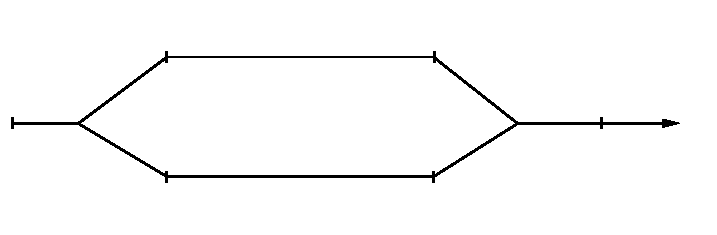
\includegraphics[width=16cm]{fig00c.eps}
  \caption{Timeline in a centralized structure}\label{fig1}
\end{figure}


  With this new setup the principal's  optimization problem becomes:
 \begin{eqnarray*}
\nonumber   && \max\limits_{q,i,f,b,F,B,D}\
\mathbb{E}_{\mathbold{\epsilon}}[u_f]=\mathbb{E}_{\mathbold{\epsilon}}\text{\Big{\{}}q+i-\lambda[f+bq+
F+Bq+Di]\text{\Big{\}}}\\
\nonumber &&\text{subject to}\\
&&\mathbb{E}_{\mathbold{\epsilon}}[u_h]=\mathbb{E}_{\epsilon_1}[-\e^{-\rho[f+bq-\frac{1}{2}\tau
a^2+z(a)]}]
\geq u_h(\bar{b})\label{ir_h}\\
&&\mathbb{E}_{\mathbold{\epsilon}}[u_m]=\mathbb{E}_{\mathbold{\epsilon}}[-\e^{-\eta[F+Bq+Di-\frac{1}{2}(\psi_1t_1^2+
\psi_2t_2^2)-\psi_{12}t_1t_2+\phi(t_1,t_2)]}] \geq u_m(\bar{w})\label{ir_m}\\
&&a\in argmax_{a}\mathbb{E}_{\epsilon_1}[-\e^{-\rho[f+bq-\frac{1}{2}\tau
a^2+z(a)]}]\label{ic_h}\\
&&t_1,t_2 \in argmax_{t_1,t_2}\mathbb{E}_{\mathbold{\epsilon}}[-\e^{-\eta[F+Bq+Di-\frac{
1}{2}(\psi_1t_1^2+ \psi_2t_2^2)-\psi_{12}t_1t_2+\phi(t_1,t_2)]}]\label{ic_m}
\end{eqnarray*}
The first two constraints are  the participation or rationality ones and the third and fourth are the incentive compatibility constraints on agents effort.  Using the first order approach and the definition of certainty equivalents \footnote{In the case of the physician we have that $\mathbb{E}_{\mathbold{\epsilon}}[u_m]=-\e^{-\eta\widehat{w}(t_1,t_2)}$, being $\widehat{w}(t_1,t_2)=F+B(\bar{a}+t_1)+Dt_2+\phi_1t_1+\phi_2t_2-\frac{1}{2}(\psi_1t_1^2+
\psi_2t_2^2)-\psi_{12}t_1t_2-\frac{\eta}{2}(B^2\sigma_1^2+D^2\sigma_2^2+2BD\sigma_{12}^2)
$, her certainty equivalent income for a given realization of $a$. For the hospital the certainty equivalent is $ \widehat{b}(a)=f+b(a+\bar{t_1})+z_1a-\frac{1}{2}\tau a^2-\frac{\rho}{2}b^2\sigma_1^2$ given values of $t_1$ and $t_2$.}, we get that:
\begin{eqnarray*}
b^C&=&\tau a-z_1\\
B^C&=&\psi_1t_1+\psi_{12}\bar{t}_2-\phi_1\\
D^C&=&\psi_2t_2 +\psi_{12}\bar{t}_1-\phi_2 \end{eqnarray*}
and solving for the \emph{second best} levels of effort derives into:
\begin{eqnarray}
a^{C}&=&\frac{b+z_1}{\tau}\label{aso}\\
t_1^{C}&=&\frac{(B+\phi_1)\psi_2-(D+\phi_2)\psi_{12}}{\psi_1\psi_2-\psi_{12}^2}\label{t1so}\\
t_{{2}}^{C}&=&\frac { \left( D+\phi_{{2}} \right) \psi_{{1}}- \left( B+\phi _{{1}} \right)
\psi_{{12}}}{\psi_1\psi_2-\psi_{12}^2}\label{t2so}
\end{eqnarray}
The principal then sets the fixed components of the payment mechanisms so as to make the participation constraints binding (which means that at the optimum  $ \bar{b}=\widehat{b} $ and $\bar{w}=\widehat{w} $) and the compensation schemes turn into:
\begin{eqnarray*}
 H(q) &=& \bar{b}+\frac{1}{2}\tau a^2-z_1a+\frac{\rho}{2}b^2\sigma_1^2\\
  M(q,i) &=& \bar{w}+\frac{1}{2}(\psi_1t_1^2+
\psi_2t_2^2)+\psi_{12}t_1t_2-\phi_1t_1-\phi_2t_2+\frac{\eta}{2}(B^2\sigma_1^2+D^2
\sigma_2^2+2DB\sigma_{12}^2)
\end{eqnarray*}
Now the optimization problem can be expressed in the following way:
\begin{eqnarray*}
\max\limits_{q,i,b,B,D}\ \mathbb{E}_{\mathbold{\epsilon}}[u_f]&=&a+t_1+t_2-\lambda(H(q)+M(q,i))\\
\nonumber \text{subject to }&&\\
a&=a^{C}=&\frac{b+z_1}{\tau}\\
t_1&=t_1^{C}=&\frac{(B+\phi_1)\psi_2-(D+\phi_2)\psi_{12}}{\psi_1\psi_2-\psi_{12}^2}\\
t_2&=t_2^{C}=&\frac { \left( D+\phi_{{2}} \right) \psi_{{1}}- \left( B+\phi _{{1}} \right)
\psi_{{12}}}{\psi_1\psi_2-\psi_{12}^2}
\end{eqnarray*}

Assuming that both random components of outputs are independently distributed ( $\sigma_{12}=0$) and solving the optimization problem of the principal we get the second-best expressions for the power of incentives:
\begin{eqnarray}
b^C&=&\frac {1}{\lambda(1+\rho\sigma_1^2\tau)}\label{bso}\\
B^C&=&\frac{\psi_2-\psi_{12}(1-\lambda D^C)}{\lambda[\psi_2+\eta\sigma_1^2(\psi_1\psi_2-
\psi_{12}^2)]}\label{Bso1}\\
D^C&=&\frac{\psi_1-\psi_{12}(1-\lambda
B^C)}{\lambda[\psi_1+\eta\sigma_2^2(\psi_1\psi_2-\psi_{12}^2)]}\label{Dso1}
\end{eqnarray}

Solving equations \ref{Bso1} and \ref{Dso1} for $B^C$ and $D^C$ we get:
\begin{eqnarray}
B^C&=&\frac{1+\eta\sigma_2^2(\psi_2-\psi_{12})}{\lambda[1+\sigma_1^2\sigma_2^2
\eta^2(\psi_1\psi_2-\psi_{12}^2)+\eta(\sigma_1^2\psi_1+\sigma_2^2\psi_2)]}\label{Bso2}\\
D^C&=&\frac{1+\eta\sigma_1^2(\psi_1-\psi_{12})}{\lambda[1+\sigma_1^2\sigma_2^2
\eta^2(\psi_1\psi_2-\psi_{12}^2)+\eta(\sigma_1^2\psi_1+\sigma_2^2\psi_2)]}\label{Dso2}
\end{eqnarray}

We can highlight a series of results in the centralized structure solution:
\begin{itemize}
  \item Unlike the first best solution, the contract design does not depend on the degree of altruism of the agents. Therefore, under asymmetric information, the optimal payment scheme is the same both for hospitals or physicians public or private.
  \item When both physicians' tasks are substitutes ($\psi_{12}>0$) the optimal power of incentives should be directly related and thus increasing the incentive payment on quantity should be realigned with an increase in variable payment on intensity.
  \item The power of incentives is independent across agents. Changing the incentives for the hospital will have no effect on the incentives of the physician.
  \item When intensity is difficult to measure (high $\sigma_2$) and efforts are perfect substitutes the optimum solution implies no power of incentives for the physician (a fixed salary) and all the power of incentives rests in the hospital payment parameter.
  %\item If  institutional or information constraints prevent the payer from using the second best incentive schemes to be applied the effort levels will differ to the ones just shown.
  \item If no incentives are used (only fixed payments schemes) the effort level of hospital will be lower than the second best solution. The physician effort will be lower or higher depending on her technology and preferences parameters (see \hl{Appendix} for proof). In particular, given that $\psi_1=\psi_2$ and $\sigma_2>\sigma_1$, then effort on intensity will be higher and effort on quantity will be lower. Fixed payments will generate below optimal quantity of cases treated and above optimal intensity of treatments.
  \item Under a financing scheme only providing optimal incentives to quantity efficiency ($b$ given by equation (\ref{bso}) and $B$ by equation (\ref{Bso2}) and $D=0$) both hospital and physician provide a higher level of effort on quantity but the physician underprovides effort on intensity.
  \item If we consider a mixed type of payment scheme including optimal power of incentives for hospital ($b^C$ in equation (\ref{bso}) ) but none  for physician ($B=D=0$) then, depending again on the parameter values, we should observe both underprovision of quantity and intensity levels.
  \item In a centralized structure we can compare multioutputs levels across different incentive payment mechanisms  in relation to a base line of pure fixed payment with no incentives (for instance the traditional retrospective or cost reimbursement system).
\end{itemize}

\subsection{Decentralized structure}

In a decentralized structure the principal (the financier) contracts only with the hospital for a certain $q$ and $i$ and then is the hospital who contracts with the physician. The assumption of asymmetric information holds in this case for the relation between hospital and physician as well. Solving by backwards induction we start with the hospital maximization problem. This amounts to finding the values of $B$,$D$ (incentive components of the physician payment) and $a$ (effort level on quantity provided by the hospital) given the parameters fixed by the principal rewarding hospital multi-output levels ($b$ and $d$). Given the second-best levels of effort levels we proceed by solving the principal's optimization problem. Figure \ref{fig2} shows the time line in this organizational structure.

%\vspace{1cm}
\begin{figure}[htbp!]
  \centering
  % Requires \usepackage{graphicx}
  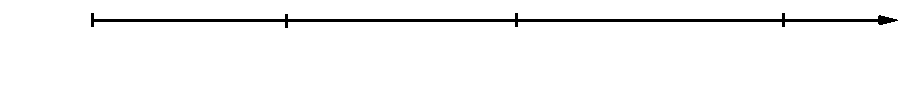
\includegraphics[width=15cm]{fig00d.eps}
  \caption{Timeline in a decentralized structure}\label{fig2}
\end{figure}

\newpage



The hospital problem expressed with the respective certainty equivalents is, therefore:
\begin{eqnarray*}
\max\limits_{a,B,D}\ \mathbb{E}_{\mathbold{\epsilon}}[u_h]&=&
f+ \left( b-B \right)  \left( a+t_{{1}} \right) + \left( d-D \right) t_{{2}}+z_{{1}}a-M\\
\nonumber \text{subject to }&&\\
t_1=t_1^{D}&=&\frac{(B+\phi_1)\psi_2-(D+\phi_2)\psi_{12}}{\psi_1\psi_2-\psi_{12}^2}\\
t_2=t_2^{D}&=&\frac {\left( D+\phi_{{2}} \right) \psi_{{1}}- \left( B+\phi _{{1}} \right)}{\psi_1\psi_2-\psi_{12}^2}\\
\hat{w}&=&\bar{w}
\end{eqnarray*}

Where  $M=\frac{\tau\,{a}^{2}}{2}+\frac{1}{2}\rho\left((b-B)^2\sigma_1^2+(d-D)^2\sigma_2^2+2(b-B)(d-D)\sigma_{12}^2
 \right)+F$ is the total hospital cost based on three components: effort cost, risk premium and the fixed term of physician payment,$F$ (this last is set so as to allow the physician achieve her reservation utility).\footnote{$F=\bar{w}-B \left( a+t_{{1}} \right) -\phi_{{1}}t_{{1}}- Dt_{{2}}-\phi_{{2}}t_{{2}}+\frac{1}{2}\,\left(\psi_{{1}}{t_{{1}}}^{2}+\psi_{{2}}{t_{{2}}}^{2}\right)
 +\psi_{{12}}t_{{1}}t_{{2}}+\frac{\eta}{2}\left( {B}^{2}{\sigma_{{1}}}^{2}+2\,BD{\sigma_{{12}}}^{2}+{D}
^{2}{\sigma_{{2}}}^{2} \right)$}

Referring to the sum of risk aversion coefficients as $\theta=(\rho + \eta)$ and $\delta={\psi_1\psi_2-\psi_{12}^2}$ the optimal variable payment components to physician are given by:
\begin{eqnarray*}
B^D&=&\frac{b(1+\sigma_1^2\rho\psi_1+\sigma_2^2\theta(\rho\delta\sigma_1^2+\psi_2))-d\eta\sigma_2^2\psi_{12}}{1+\psi_1
\theta\sigma_1^2+\theta\sigma_2^2\left(\theta\delta\sigma_1^2+\psi_2\right)}\\
D^D&=&\frac{d(1+\sigma_2^2\rho\psi_2+\sigma_1^2\theta(\rho\delta\sigma_2^2+\psi_1))-b\eta\sigma_2^2\psi_{12}}{1+\psi_2
\theta\sigma_2^2+\theta\sigma_1^2\left( \theta\,\delta\sigma_2^2+\psi_1\right)}
\end{eqnarray*}
By solving for $t_1$ and $t_2$ given values of $B$ and $D$ we obtain the second best physician efforts $t_1(b,d)$ and $t_2(b,d)$ that the hospital will incentivize as function of his own payment parameters.

The principal's optimization problem now is given by:
\begin{eqnarray*}
% \nonumber % Remove numbering (before each equation)
  \max\limits_{q,i,b,d}\ \mathbb{E}_{\mathbold{\epsilon}}[u_f]&=&a+t_1+t_2-\lambda\left (f+b(a+t_1)+dt_2\right ) \\
  a^D&=&\frac{b+z_1}{\tau}\\
  t_1^D &=& t_1(b,d) \\
  t_2^D &=& t_2(b,d)\\
  \hat{b}&=&\bar{b}
\end{eqnarray*}
where $f=\bar{b}-(b-B)(a+t_1)-(d-D)t_2-z_1a-M$ is the fixed component of the hospital scheme that makes his participation constraint binding. The solution to this program is a complicated object that  depends on the fundamental parameters. For the special case of independent tasks in the physician's cost function ($\psi_{12}=0$) the optimal payment parameters on the variable components are set by hospital and principal according to these expressions:
\begin{eqnarray*}
% \nonumber % Remove numbering (before each equation)
  B^D &=& {\frac { \left( {\sigma_{{1}}}^{2}\theta\,{\psi_{{1}}}^{2}+ \left(
\rho\,\tau\,{\sigma_{{1}}}^{2}+1 \right) \psi_{{1}}+\tau \right)
 \left( \rho\,\psi_{{1}}{\sigma_{{1}}}^{2}+1 \right) }{ \left( {\sigma
_{{1}}}^{2} \left( \eta\,\rho\,\tau\,{\sigma_{{1}}}^{2}+\eta+\rho
 \right) {\psi_{{1}}}^{2}+ \left( \rho\,\tau\,{\sigma_{{1}}}^{2}+1
 \right) \psi_{{1}}+\tau \right) \lambda\, \left( {\sigma_{{1}}}^{2}
\theta\,\psi_{{1}}+1 \right) }} \\
  D ^D&=& {\frac { \left( \rho\,\psi_{{2}}{\sigma_{{2}}}^{2}+1 \right) ^{2}}{
\lambda\, \left( {\sigma_{{2}}}^{2}\theta\,\psi_{{2}}+1 \right)
 \left( \eta\,\rho\,{\psi_{{2}}}^{2}{\sigma_{{2}}}^{4}+\rho\,\psi_{{2}
}{\sigma_{{2}}}^{2}+1 \right) }}\\
  b^D &=& {\frac {{\sigma_{{1}}}^{2}\theta\,{\psi_{{1}}}^{2}+ \left( \rho\,\tau
\,{\sigma_{{1}}}^{2}+1 \right) \psi_{{1}}+\tau}{ \left( {\sigma_{{1}}}
^{2} \left( \eta\,\rho\,\tau\,{\sigma_{{1}}}^{2}+\eta+\rho \right) {
\psi_{{1}}}^{2}+ \left( \rho\,\tau\,{\sigma_{{1}}}^{2}+1 \right) \psi_
{{1}}+\tau \right) \lambda}}\\
  d^D &=& {\frac {\rho\,\psi_{{2}}{\sigma_{{2}}}^{2}+1}{ \left( 1+ \left( \eta
\,{\psi_{{2}}}^{2}{\sigma_{{2}}}^{4}+\psi_{{2}}{\sigma_{{2}}}^{2}
 \right) \rho \right) \lambda}}
%B^D&=&{\frac { \left(  \left( \tau+\psi_{{1}} \right) \rho+\eta\,\psi_{{1}}
% \right) \rho}{\lambda\, \left(  \left( \eta\,\tau\,\psi_{{1}}{\sigma_
%{{1}}}^{2}+\tau+\psi_{{1}} \right) {\rho}^{2}+\eta\,\psi_{{1}} \left(
%\eta\,\tau\,{\sigma_{{1}}}^{2}+2 \right) \rho+{\eta}^{2}\psi_{{1}}
% \right) }}\\
% D^D&=&{\frac {\rho}{\lambda\, \left(  \left( \eta\,\psi_{{2}}{\sigma_{{2}}}^
%{2}+1 \right) \rho+{\eta}^{2}\psi_{{2}}{\sigma_{{2}}}^{2} \right) }}\\
%b^D&=&{\frac { \left(  \left( \tau+\psi_{{1}} \right) \rho+\eta\,\psi_{{1}}
% \right) \theta}{\lambda\, \left(  \left( \eta\,\tau\,\psi_{{1}}{
%\sigma_{{1}}}^{2}+\tau+\psi_{{1}} \right) {\rho}^{2}+\eta\,\psi_{{1}}
% \left( \eta\,\tau\,{\sigma_{{1}}}^{2}+2 \right) \rho+{\eta}^{2}\psi_{
%{1}} \right) }}\\
%d^D&=&{\frac {\theta}{\lambda\, \left(  \left( \eta\,\psi_{{2}}{\sigma_{{2}}
%}^{2}+1 \right) \rho+{\eta}^{2}\psi_{{2}}{\sigma_{{2}}}^{2} \right) }}
\end{eqnarray*}

As we can see, altruistic parameters do not enter the payment component as was in the centralized structure. The optimal effort levels for both the hospital and the physician are\footnote{To compact the solution we  will assume there is no altruistic interest in both hospital and physician, i.e. $z_1=\phi_1=\phi_2=0$}.

%%%$\alpha_0=\eta\,\lambda\,\tau\,{\sigma_{{1}}}^{2}z_{{1}}\,, \alpha_1=\eta\,\lambda\,\tau\,\phi_{{1}}{\sigma_{{1}}}^{2}$ and $\alpha_2=\eta\,\lambda\,\phi_{{2}}\psi_{{2}}{\sigma_{{2}}}^{2}$}:
%
%
\begin{eqnarray*}
a^D&=&{\frac {{\sigma_{{1}}}^{2}\theta\,{\psi_{{1}}}^{2}+ \left( \rho\,\tau
\,{\sigma_{{1}}}^{2}+1 \right) \psi_{{1}}+\tau}{\tau\,\lambda\,
 \left( {\sigma_{{1}}}^{2} \left( \eta\,\rho\,\tau\,{\sigma_{{1}}}^{2}
+\eta+\rho \right) {\psi_{{1}}}^{2}+ \left( \rho\,\tau\,{\sigma_{{1}}}
^{2}+1 \right) \psi_{{1}}+\tau \right) }}\\
t_1^D&=&{\frac { \left( \rho\,\psi_{{1}}{\sigma_{{1}}}^{2}+1 \right)  \left( {
\sigma_{{1}}}^{2}\theta\,{\psi_{{1}}}^{2}+ \left( \rho\,\tau\,{\sigma_
{{1}}}^{2}+1 \right) \psi_{{1}}+\tau \right) }{\lambda\,\psi_{{1}}
 \left( \theta\,\psi_{{1}}{\sigma_{{1}}}^{2}+1 \right)  \left( {\sigma
_{{1}}}^{2} \left(  \left( \eta\,\tau\,{\sigma_{{1}}}^{2}+1 \right)
\rho+\eta \right) {\psi_{{1}}}^{2}+ \left( \rho\,\tau\,{\sigma_{{1}}}^
{2}+1 \right) \psi_{{1}}+\tau \right) }}\\
t_2^D&=& {\frac { \left( \rho\,\psi_{{2}}{\sigma_{{2}}}^{2}+1 \right) ^{2}}{
\lambda\,\psi_{{2}} \left( 1+ \left( \eta\,{\psi_{{2}}}^{2}{\sigma_{{2
}}}^{4}+\psi_{{2}}{\sigma_{{2}}}^{2} \right) \rho \right)  \left( \eta
\,\psi_{{2}}{\sigma_{{2}}}^{2}+\rho\,\psi_{{2}}{\sigma_{{2}}}^{2}+1
 \right) }}
% \nonumber % Remove numbering (before each equation)
  %a^{D} &=& {\frac { \left( \alpha_0+ \left( \lambda\,z_{{1}}+1 \right)  \left( \tau+\psi_{{1}} \right)
% \right) {\rho}^{2}+\eta\, \left( \alpha_0+2\,\lambda\,\psi_{{1}}z_{{1}}+\tau+2\,\psi_{{1}}
% \right) \rho+{\eta}^{2}\psi_{{1}} \left( \lambda\,z_{{1}}+1 \right) }
%{\tau\, \left(  \left( \eta\,\tau\,\psi_{{1}}{\sigma_{{1}}}^{2}+\tau+
%\psi_{{1}} \right) {\rho}^{2}+\eta\,\psi_{{1}} \left( \eta\,\tau\,{
%\sigma_{{1}}}^{2}+2 \right) \rho+{\eta}^{2}\psi_{{1}} \right) \lambda}
%}
%\\
%  t_1^{D} &=& {\frac { \left( \alpha_1+ \left( \lambda\,\phi_{{1}}+1 \right)  \left( \tau+\psi_{{1}}
% \right)  \right) {\rho}^{2}+\eta\,\psi_{{1}} \left( 2\,\lambda\,\phi_
%{{1}}+\alpha_{{1}}+1 \right) \rho+{\eta}^{2}\lambda\,\phi_{{1}}\psi_{{
%1}}}{ \left(  \left( \eta\,\tau\,\psi_{{1}}{\sigma_{{1}}}^{2}+\tau+
%\psi_{{1}} \right) {\rho}^{2}+\eta\,\psi_{{1}} \left( \eta\,\tau\,{
%\sigma_{{1}}}^{2}+2 \right) \rho+{\eta}^{2}\psi_{{1}} \right) \psi_{{1
%}}\lambda}}
%\\
%  t_2^D &=& {\frac { \left( \lambda\,\phi_{{2}}+\alpha_{{2}}+1 \right) \rho+{\eta}
%\,\alpha_{{2}}}{\psi_{{2}}
% \left(  \left( \eta\,\psi_{{2}}{\sigma_{{2}}}^{2}+1 \right) \rho+{
%\eta}^{2}\psi_{{2}}{\sigma_{{2}}}^{2} \right) \lambda}}
\end{eqnarray*}
If we compare this results with the ones in the  centralized structure:
\begin{eqnarray*}
% \nonumber % Remove numbering (before each equation)
  a^C &=& {\frac {1}{\lambda\, \left( \rho\,\tau\,{\sigma_{{1}}}^{2}+1 \right)
\tau}}\\
  t_1^C &=& {\frac {1}{ \left( \eta\,\psi_{{1}}{\sigma_{{1}}}^{2}+1 \right)
\lambda\,\psi_{{1}}}} \\
  t_2^C &=& {\frac {1}{\psi_{{2}}\lambda\, \left( \eta\,\psi_{{2}}{\sigma_{{2}}}^{
2}+1 \right) }}
\end{eqnarray*}
we can observe that the centralized structure derives much more simple solutions for the incentive payments. It can be shown (see \hl{Appendix}) that the effort level for the hospital is larger in the decentralized structure ($a^D>a^C$), whereas the intensity effort level for the physician is lower ($t_2^D<t_2^C$).  For the physician's effort on quantity to be lager under the centralized structure it will have to be that $\eta\tau\sigma_1^2>1+\sigma_1^2\theta\psi_1$. This means that given $\sigma_1$ and agents' coefficients of risk aversion ($\eta$ and $\rho$), for a sufficiently higher cost of producing $q$ on the part of the hospital relative to that same cost by the physician, the quantity provided by the physician in a centralized structure will be larger than that of a decentralized one\footnote{However, it is immediate to see that when $\psi_1>\tau$ then $t_1^D>t_1^C$.}. In other words, when tasks are independent in the physician's cost function and her marginal cost attending more patients is sufficiently lower than that of the hospital, a centralized structure with incentive compatible schemes will show more intensity in treatments and larger volume of patients taken care of. Notwithstanding the foregoing, we are interested in a richer comparison between agents' performance in different organizational settings. Using given values in the fundamental parameters of the model we will now proceed to analyze, by means of graphical illustrations, the differential power of incentives and effort outcomes between the two forms of structuring contract relations.

\section{Comparing organizational structures}
The complex form of the solution (especially in the decentralized case) does not allow for a neat  comparison of interrelations between optimal incentive schemes and optimal effort levels in both hierarchical frameworks. In order to derive some general results about the nature of tasks interdependence or the effect of noise variations in the measure of quantity or intensity we will work with  graphical simulations for different scenarios\footnote{All graphs are constructed for unit values in all the remainder parameters except when otherwise indicated. }. Let's first consider the effect of a change in $\psi_{12}$ both in the incentive parameters and in the difference between effort levels. Then we will consider (mainly for substitutive efforts) the change in $\sigma_1$ and $\sigma_2$ (the accuracy in outcomes signals).

\subsection{Change in the interaction between tasks}
Figure \ref{fig3} represents the optimal incentive payments for a grid of values of $\psi_{12}$ ranging from perfect complementarity to perfect substitution

\begin{figure}[htbp!]
  \centering
  % Requires \usepackage{graphicx}
  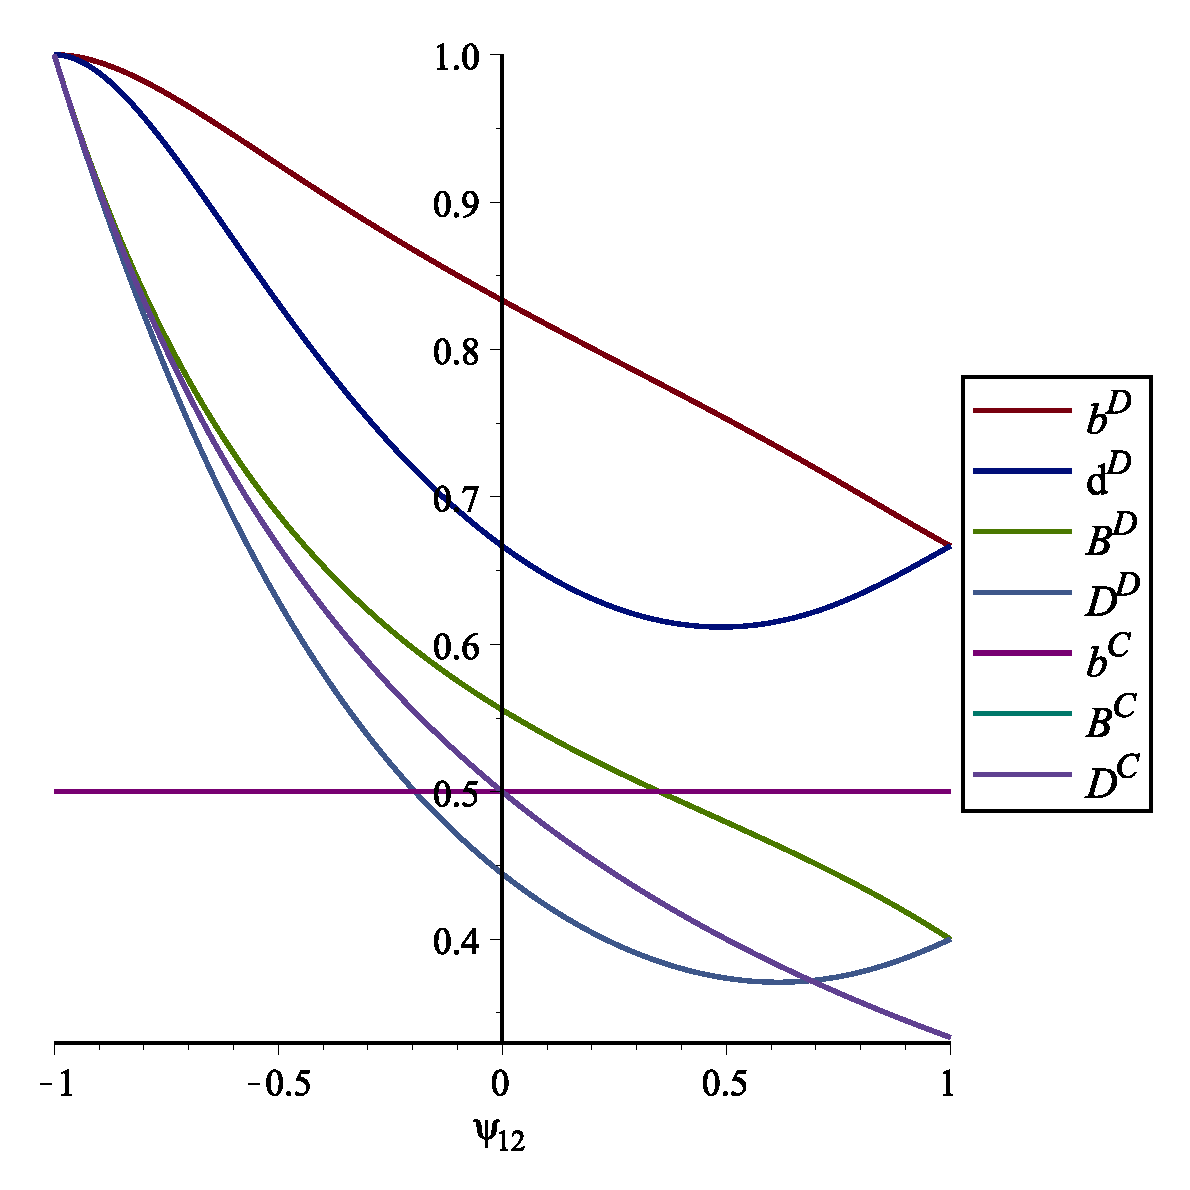
\includegraphics[width=8cm]{gr1.eps}\\
  \caption{Optimal incentives with decentralized (D) and centralized structures (C) }\label{fig3}
\end{figure}

Except for the constant incentive payment to the hospital when the principal only contracts quantity from him,  all variable payments change with the interaction between physicians tasks. When efforts are \emph{perfect complements }incentive mechanisms reach their maximum (and turn to be equal among them) in both structures. The optimal payment to hospital's quantity in the decentralized structure and the one to physician's effort on quantity in both frameworks decrease continuously as $\psi_{12}$ increase. However, payments for intensity (both for the hospital or the physician) start to increase as soon as the degree of substitution reaches a certain threshold. When the principal only contracts with the hospital the power of incentives (both for hospital and physician) is higher in the quantity dimension than in the intensity dimension (except for the extreme cases of perfect complements or perfect substitutes). Even more interestingly, although in the centralized structure all variable payments to physician tend to zero when tasks tend to perfect substitution, this is not the case in the decentralized one. As a consequence, when efforts become \emph{perfect substitutes }it is optimal for the financer (the public provider or the insurance company) not to include incentives in the physician contract  if the setup is centralized. On the contrary, when dealing exclusively with the hospital the principal will include high-powered incentive schemes that will, subsequently, \emph{cascade down }to the second tier of arrangements between hospital and physician. This result might help us see why it could be optimal to introduce performance payments for physicians whenever hospital's see their degree of autonomy being raised. On the contrary, fixed salaries or low-powered incentives shall be preferred when the principal contracts separately with hospital manager's and physician's. \emph{If tasks are perfect substitutes, somehow, the adequacy   of using incentives under moral hazard seems to be dependent on the organizational design in use.}

When this distinct  power of incentives is translated into effort levels we can best realize the differential effect  of the two organizational arrangements. Figure \ref{fig4} shows the differences in optimal effort levels in the decentralized structure over the centralized one. As seen, hospital level of quantity is always higher in a decentralized setting whereas  physician effort on quantity is only slightly superior in the centralized structure for very low (and negative) values of $\psi_{12}$. When tasks complementarity is total, efforts by physician both in quantity and intensity  is the same in both settings. As the physician efforts become more and more substitutes her performance in quantity increases in the decentralized scenario compared to the centralized one and the opposite is true for the intensity dimension.

\begin{figure}[htbp!]
  \centering
  % Requires \usepackage{graphicx}
  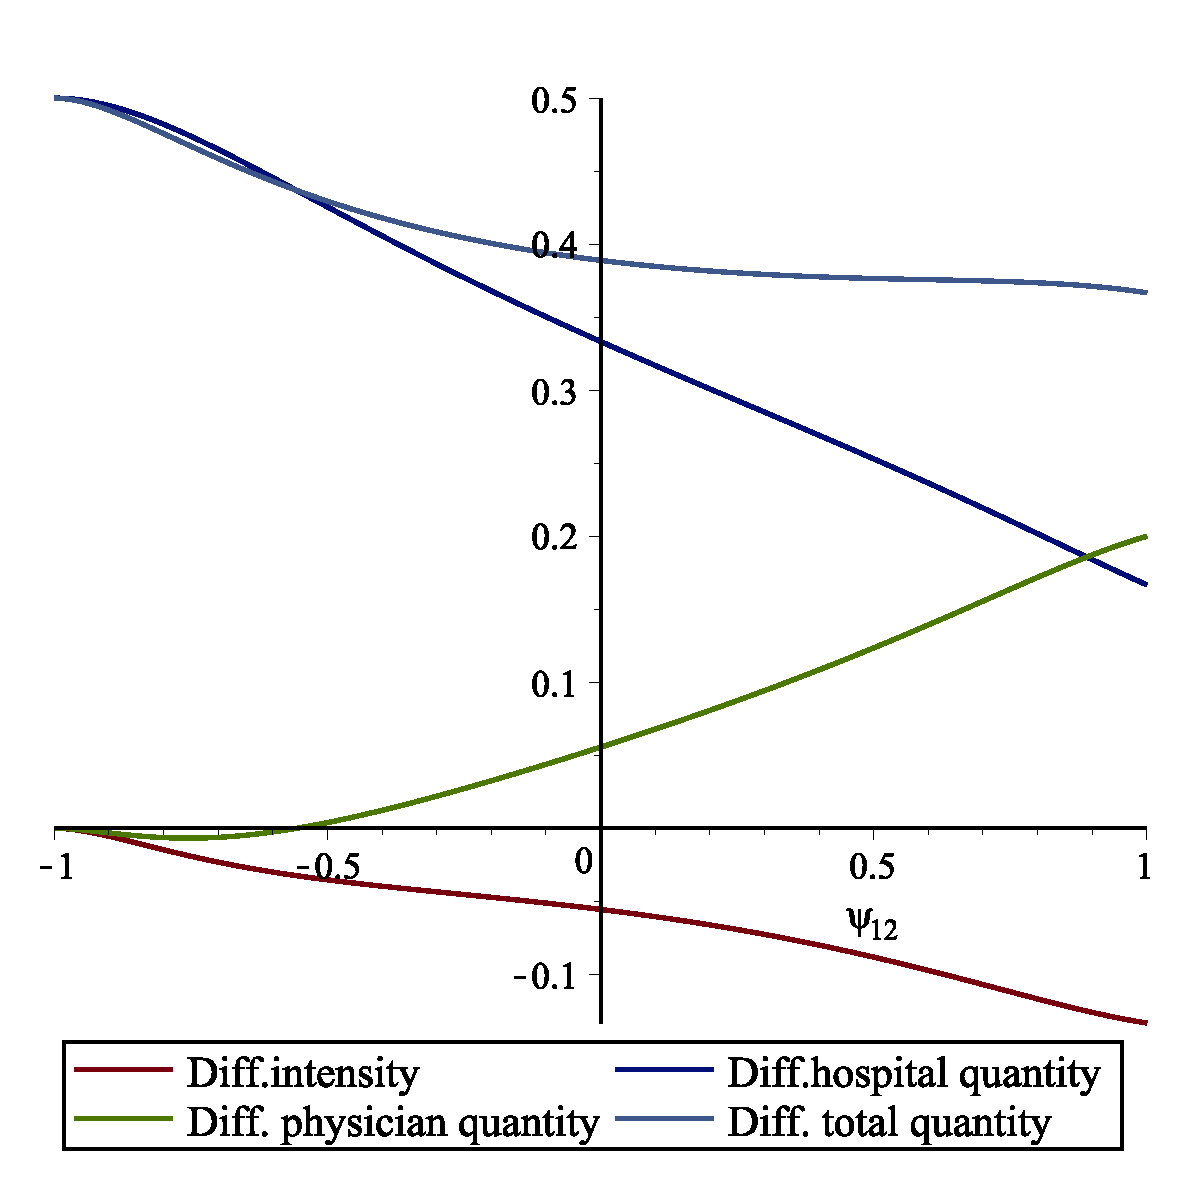
\includegraphics[width=8cm]{gr2.eps}\\
  \caption{Differential of efforts (decentralized vs. centralized)}\label{fig4}
\end{figure}

Total level of effort in quantity is higher when the principal only contracts with the hospital. As the tasks become more and more substitutes the decentralized structure shifts weights in favor of contracting quantity from physician instead of the hospital and the centralized scenario does . This should be the result of a centralized structure that reduces the power of incentives with $\psi_{12}$,  as shown above.

If the quantity level is fully determined by the effort level of the agents, that is $\sigma_1=0$,   intensity keeps being lower in the decentralized case but now the difference in effort levels on quantity, both from hospital and physician, completely offset each other so that total quantity is the same in the two structures and achieves first-best values. On the other hand, when  it is the intensity of treatment the one measured without any noisy signal ($\sigma_2=0$), quantity inputs are larger in the decentralized structure both for hospital and physician and independent of the interaction between tasks and now intensity is the same to the symmetric information scenario in both structures. Figures  \ref{fig5} and \ref{fig6} present these two special cases respectively.

\begin{figure}[htbp!]
  \centering
  % Requires \usepackage{graphicx}
  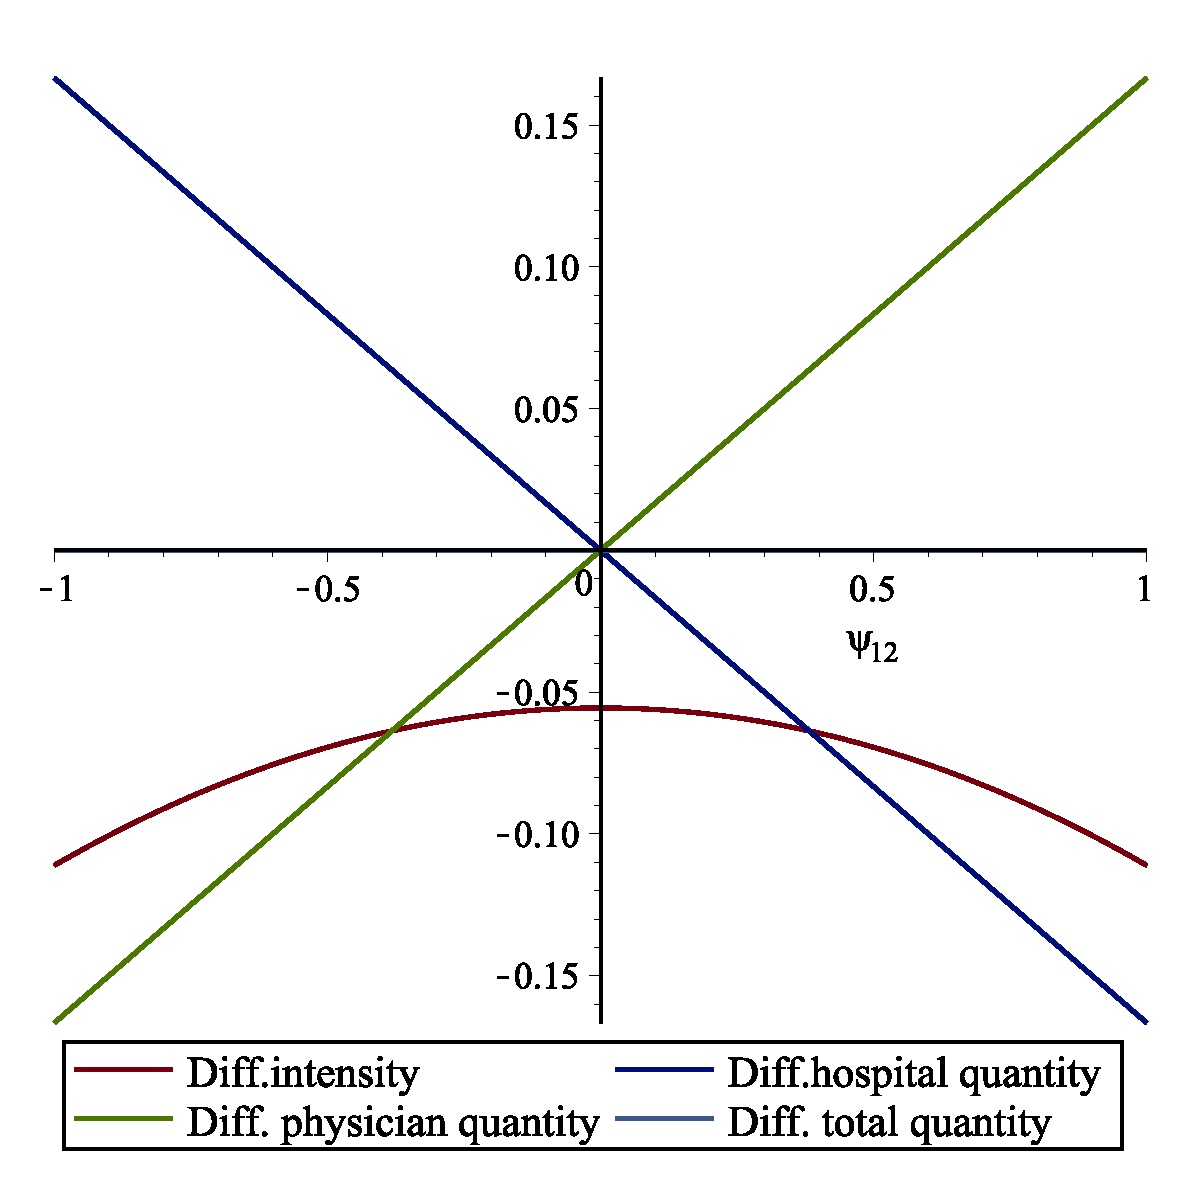
\includegraphics[width=8cm]{gr3.eps}\\
  \caption{Differential of efforts given $\sigma_1=0$}\label{fig5}
\end{figure}
\begin{figure}[htbp!]
  \centering
  % Requires \usepackage{graphicx}
  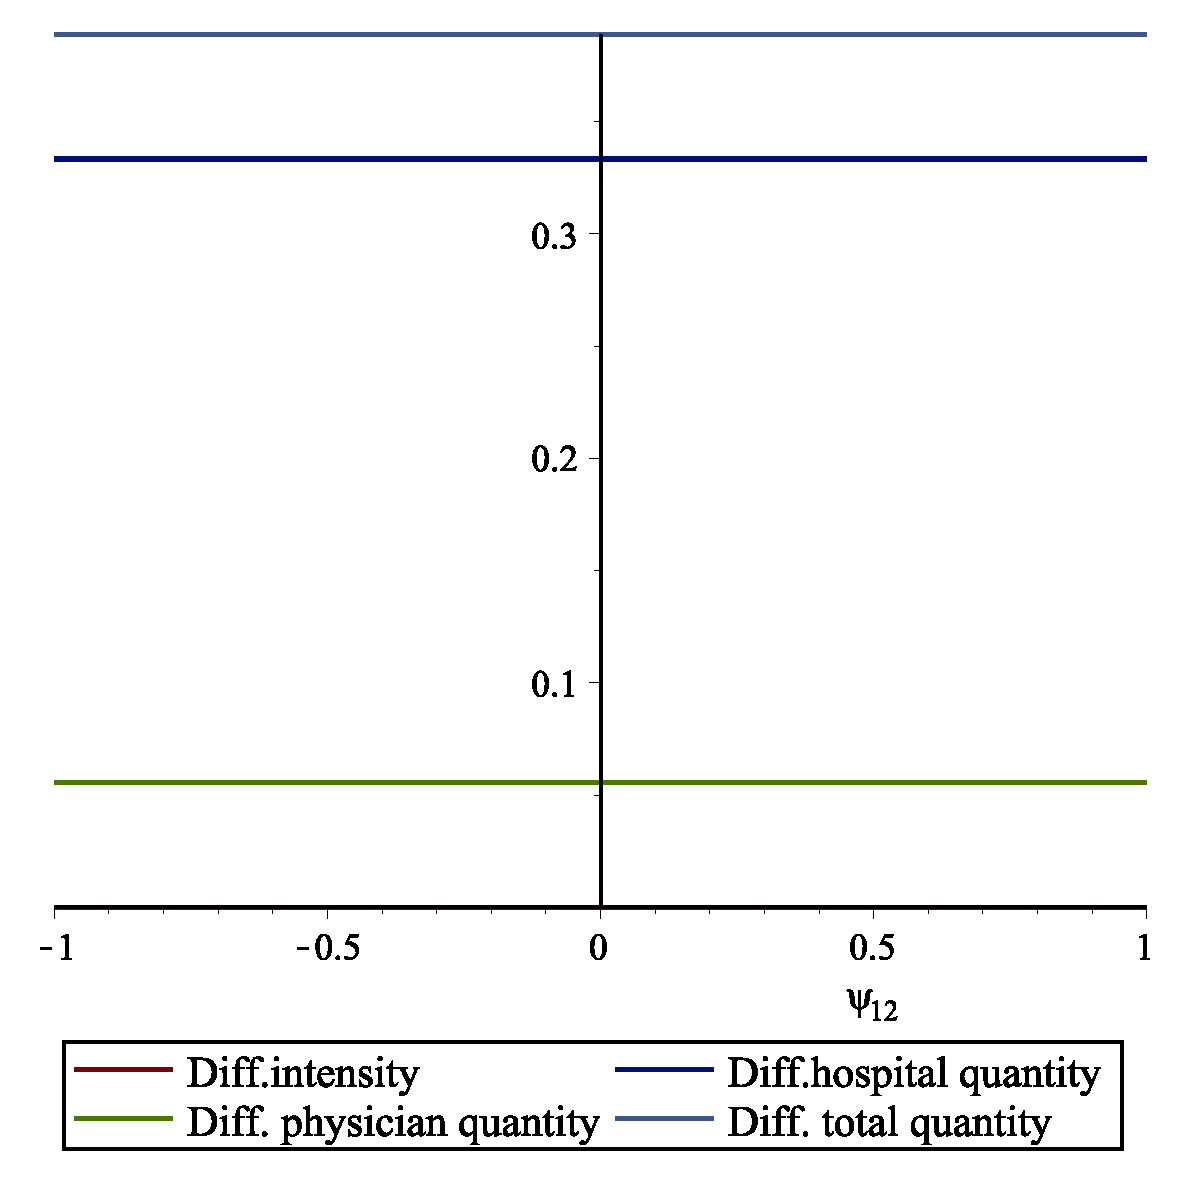
\includegraphics[width=8cm]{gr4.eps}\\
  \caption{Differential of efforts given $\sigma_2=0$.}\label{fig6}
\end{figure}
%\newpage

\subsection{Imprecise measurement of outcomes}

Let's now consider the variation in  the incentive schemes and the effort levels when, for a given value of $\psi_{12}$, the measurement of outcomes become more and more imprecise. Figure \ref{fig7} shows how the variable incentive payments change as the quantity becomes noisier and the physician's tasks are imperfect substitutes ($\psi_{12}=0.5$). All incentive parameters decrease as $\sigma_1$ increases but whereas the variable payments for quantity tend to zero, the payments for intensity stabilize asymptotically in a positive value regardless of the organizational setup. In short, as the measurement of quantity becomes more and more imprecise (therefore transferring more risk to the agents in that output dimension) the power of incentives, as expected, decrease. Incentives also decrease in the intensity outcome but then, asymptotically, tend to remain positive and constant.
\begin{figure}[htbp!]
  \centering
  % Requires \usepackage{graphicx}
  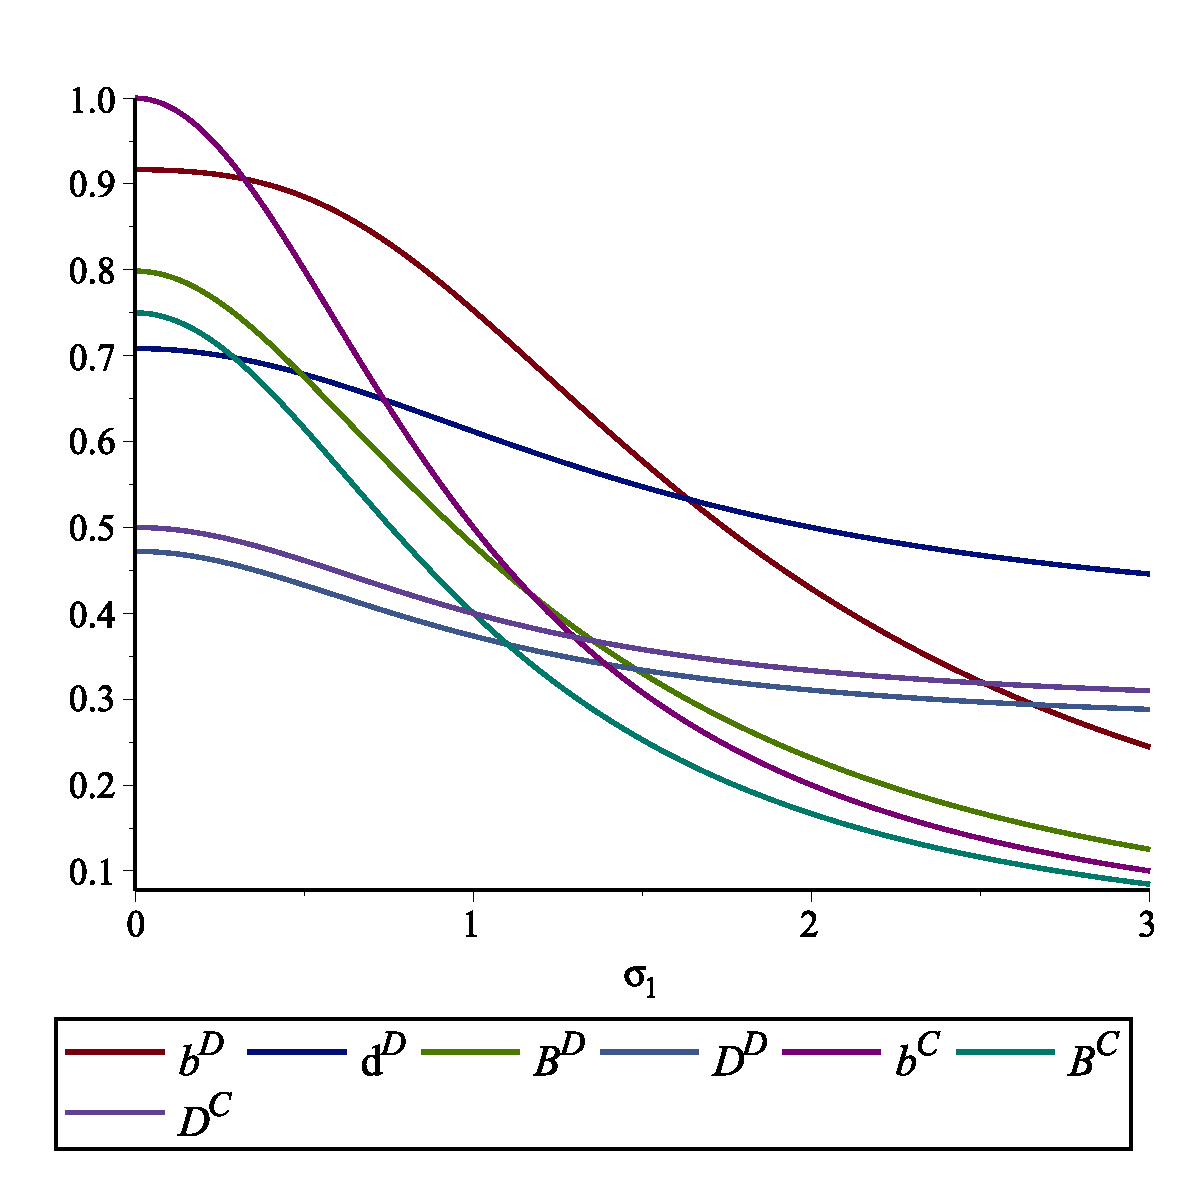
\includegraphics[width=8cm]{gr5.eps}\\
  \caption{Optimal incentives when $\sigma_1$ increases.}\label{fig7}
\end{figure}

\begin{figure}[h!]
  \centering
  % Requires \usepackage{graphicx}
  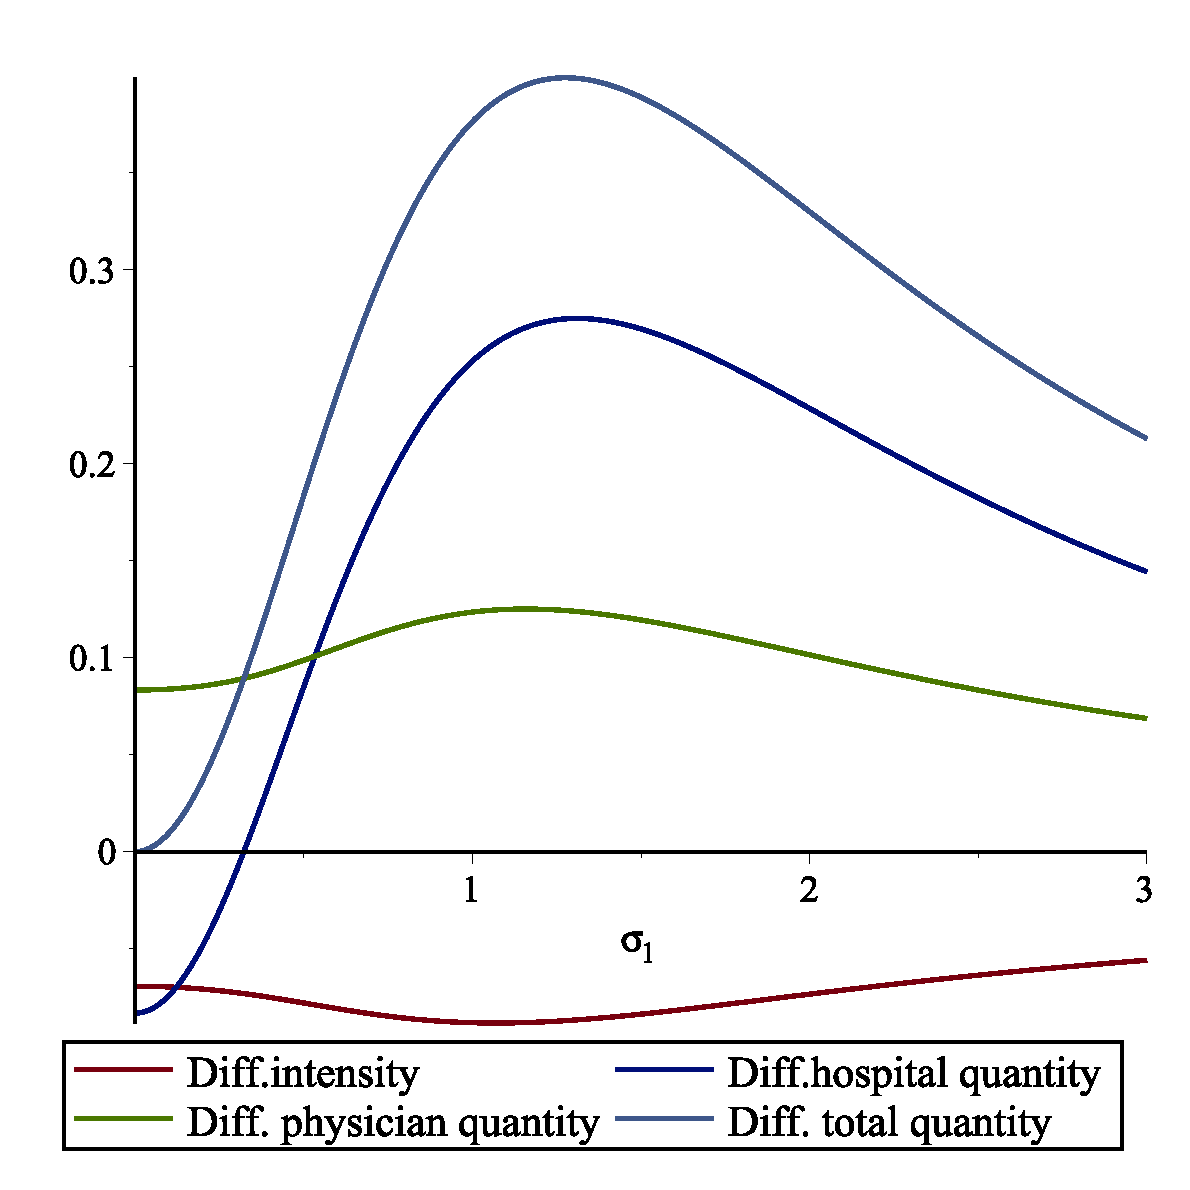
\includegraphics[width=8cm]{gr6.eps}\\
  \caption{Differential of efforts when $\sigma_1$ increases.}\label{fig8}
\end{figure}






Given these incentive schemes the difference of efforts are represented in Figure \ref{fig8}. Intensity remains higher under a centralized structure but total quantity is higher with a decentralized one. In the limit, hospital quantity efforts tend to converge in the two settings  but physician's effort on quantity stays higher in a decentralized structure no matter how large the noise in quantity measurement is. This higher effort on quantity by the physician in the decentralized case is the only force driving to a greater level of quantity in that setup\footnote{For the case of imperfect complements, however, both effort on quantity and intensity become, in the limit, higher in the centralized structure as the noise in quantity measurement grows. }.

Now we can check the effect on incentives and performance when, for given values of the rest of parameters, the noise in the measurement of intensity ($\sigma_2$) becomes larger.
Figure \ref{fig9} shows how all intensity incentives decrease and tend to zero (faster for the physician than the hospital) when $\psi_{12}=0.5$. Quantity incentives tend to diminish as noise in intensity increases (except for hospital's parameter in the centralized case which is independent of $\sigma_2$) but for high levels of imprecision in the  intensity signal they all tend to stabilize and remain positive\footnote{The opposite happens when tasks are imperfect complements and $\psi_{12}=-0.5$: incentives for quantity tend to zero with $\sigma_2$ and incentives to intensity remain positive. }.
It can be checked, however, that the sum of incentive powers on both agents is higher in the decentralized structure than in the centralized one\footnote{Interestingly, when tasks become almost perfect substitutes, the power of incentives in the decentralized case tend to zero as the imprecision in intensity values grows larger}.

\begin{figure}[htbp!]
  \centering
  % Requires \usepackage{graphicx}
  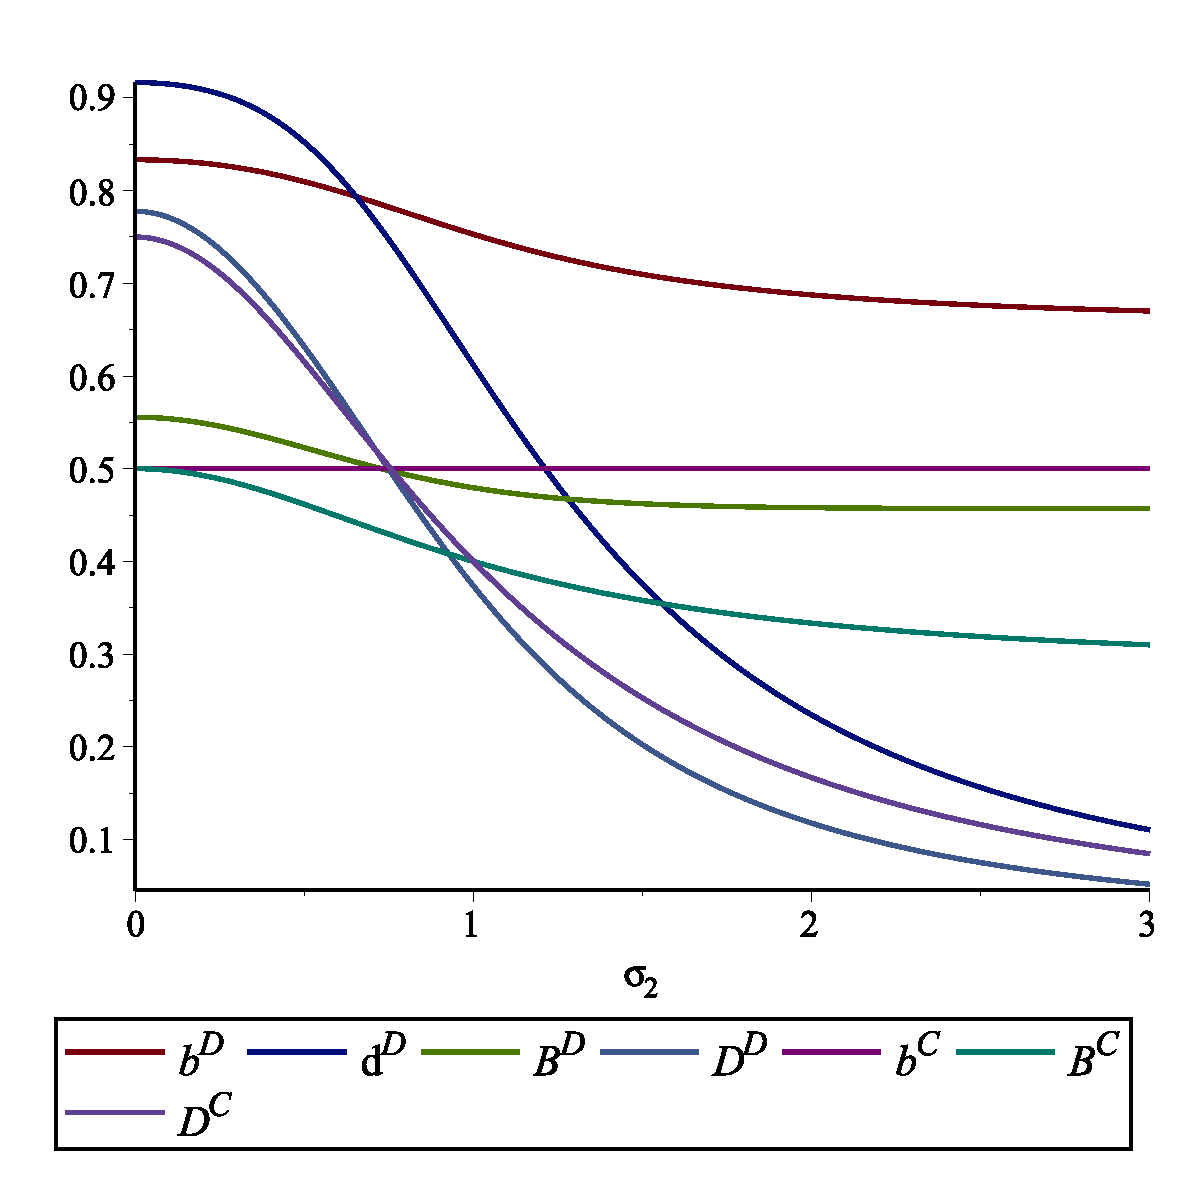
\includegraphics[width=8cm]{gr7.eps}\\
  \caption{Optimal incentives when $\sigma_2$ increases.}\label{fig9}
\end{figure}



The interaction of these incentive schemes with the rest of the parameters of the model gives rise to a profile of difference in effort performance between organizations that can be visually analyzed in Figure \ref{fig10}.

For mid-range substitution level between tasks ($\psi_{12}=0,5$) when intensity is measured without noise physician's levels of $t_2$ are equal and both physician and hospital effort on quantity are larger in the decentralized case. But as long as $\sigma_2$ tends to become larger, intensity is reduced in the decentralized case with respect to the centralized structure. Quantity effort for hospital decreases and physician's one decreases but they both continue to remain higher when the principal only contracts with the hospital.
\begin{figure}[htbp!]
  \centering
  % Requires \usepackage{graphicx}
  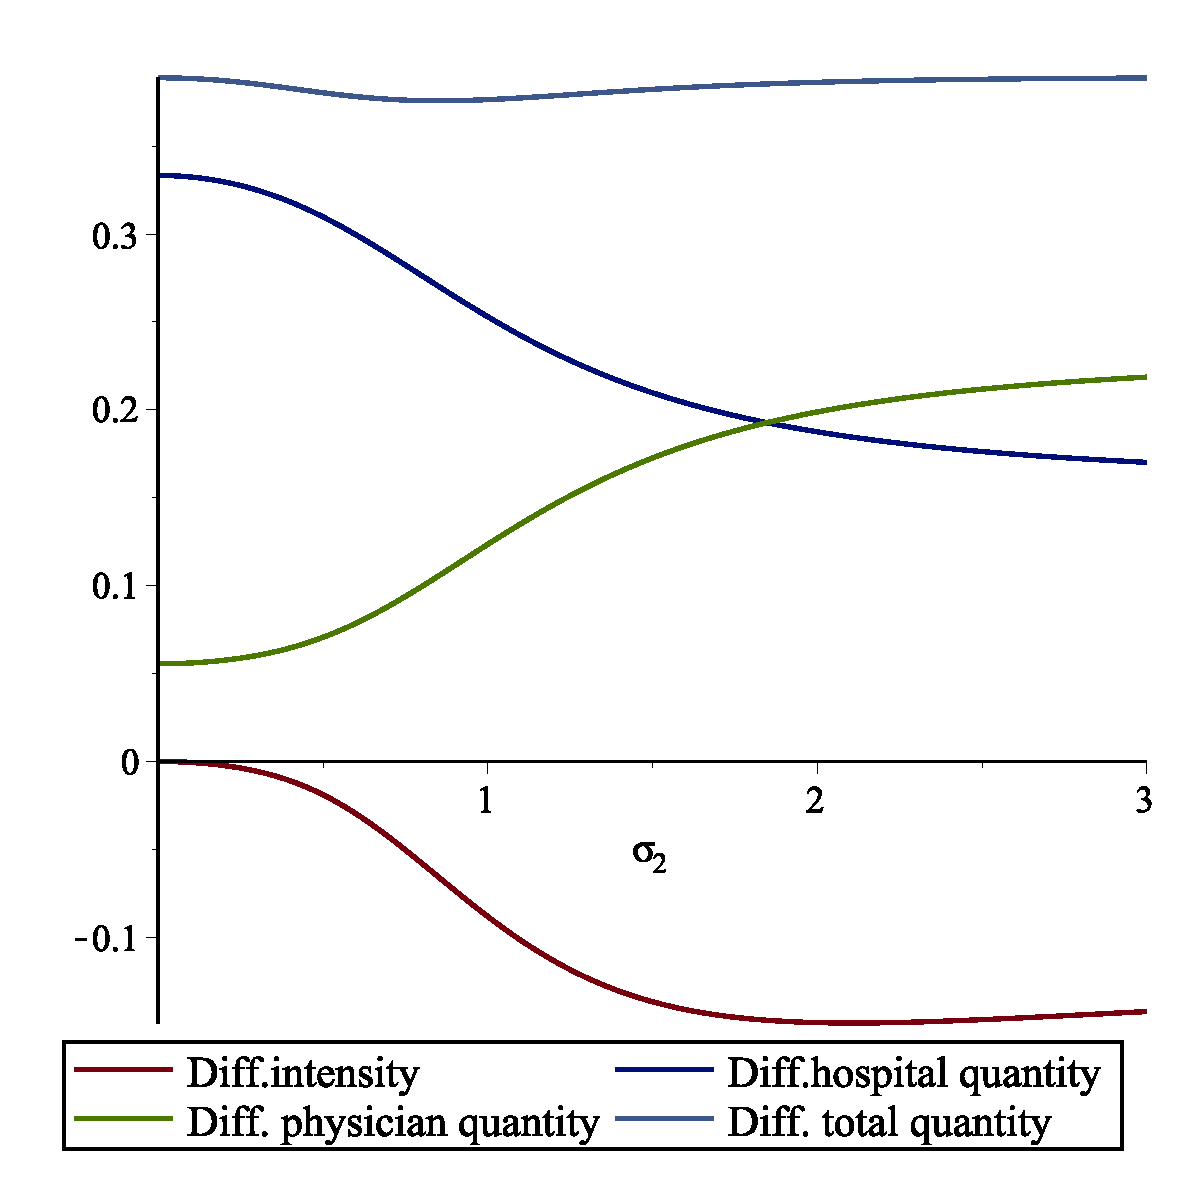
\includegraphics[width=8cm]{gr8.eps}\\
  \caption{Differential of efforts when $\sigma_2$ increases and tasks are imperfect substitutes ($\psi_{12}=0.5$).}\label{fig10}
\end{figure}

\begin{figure}[htbp!]
  \centering
  % Requires \usepackage{graphicx}
  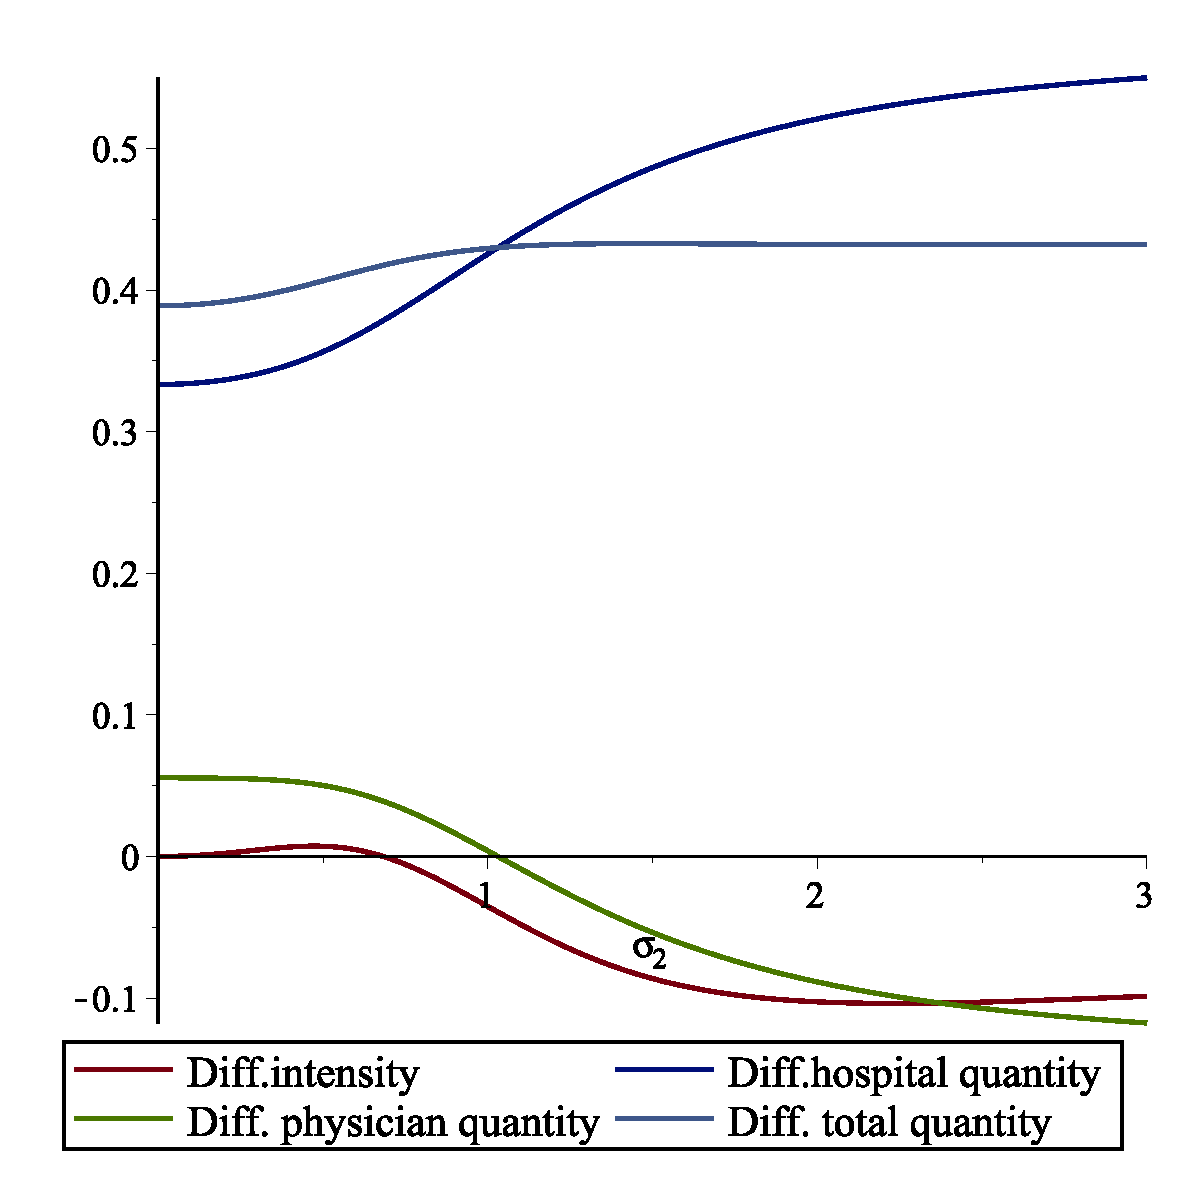
\includegraphics[width=8cm]{gr9.eps}\\
  \caption{Differential of efforts when $\sigma_2$ increases and tasks are imperfect complements ($\psi_{12}=-0.5$).}\label{fig11}
\end{figure}



It might be interesting to check how much of  this variation in performance depends upon the interaction between tasks. Figure \ref{fig11} represents the same results in efforts differences for complementary tasks in the physician cost function. The most remarkable finding is that now the initial effect on hospital and physician quantity efforts are reversed (physician effort decreases and hospital increases in the decentralized structure) and when $\sigma_2$ becomes slightly larger than $\sigma_1$ physician's effort on quantity starts to be bigger in the centralized structure than in the decentralized one.\footnote{Combining this result with the switch in effects on agents quantities we can see how when $\sigma_1=0$ (perfect measurement of quantity) quantity is the same in both organizational setups but intensity is always higher in the centralized one. }


\section{Conclusions}
In the previous pages we have tried to characterize the main features of a model of health care provision in a multiple-agents, multiple-outputs setup. To that aim we have stressed the relevance of the information and organizational structure and the links between these two. The purpose is to obtain some relevant results in terms of optimal power of incentives and efforts exerted by agents thereof. The informational constraint considered is one of a moral hazard type and in both the hospital managers and in the physicians. The mayor bottom line to be analyzed is how introducing incentives in the financing of hospitals has different output consequences depending on the structure of the organization being in effect.

In a symmetric information benchmark, we have shown that the principal uses lump-sum payments as first-best solutions and keeps the agents with their reservation utilities.  No power of incentives are included in the optimal contract. Furthermore, physician and hospital equalize marginal costs  on quantity production and that the marginal rate of substitution for the principal between quantity and intensity must be equal to the marginal rate of transformation between tasks. One of the implications of the first-best solution is the direct relation between the degree of altruism on the agent and the effort level required.

Once the benchmark is established we have proceeded by studying the case of hidden actions and moral hazard under two organizational structures: a centralized contracting (the principal deals simultaneously with hospital and physicians) and a decentralized one (the payer only hires services from the hospital and the hospital autonomously designs the contract for physician services). The main feature of the model specification is that while the physician exerts effort in the two dimensions (being these independent, complements or substitutes in the cost function) the hospital only takes decisions on the quantity of patients to be treated. In order to derive closed form solutions we, accordingly, specified CARA type utility functions on the agents, normally distributed performances and linear incentive schemes. The general result in the literature shows \emph{incentives complementarity }whenever there are effort-substitution problems\footnote{See \cite{Bolton05}, page 222.}. This result, however, has to be qualified in our model since that turns only to be the case in the decentralized structure. When the principal contracts quantity from the hospital and the physician alike, the incentives complementarity only applies to the physician contract while the hospital power of incentives remain constant and independent of the substitution of efforts. In a way, by giving autonomy to the hospital we get him to internalize the effort-substitution problem and, thus, the principal has to take it into account in the hospital incentives scheme derived from a backwards induction setup.

More interestingly, we study how the agents'  incentive parameters turn out to vary  in the two organizational settings and the final outcome levels response thereby.
Both in the centralized and decentralized structures the optimal power of incentives do not depend on the altruism or vocational component of the agents. In the centralized structure  incentives are independent across agents whereas in the decentralized one they are connected by construction. %However, for high degrees of substitution both variable payments move in the opposite direction.

 %When the quality of intensity measure worsens incentives to quantity and intensity tend to vanish for physician in both structures if tasks are perfect substitutes. This is also the case for the hospital in the decentralized setup but not in the centralized one (again, we can see it as the principal's best response to the hospital enlarged power of decision). The corollary then is that under a noisy signal in the intensity of treatment the second best contract implies only fixed payments to both health-care providers in the decentralized case and only considers variable components to the hospital when the structure is centralized.

 Under a centralized organization (the most common in the Spanish hospital system) we show how different financing mechanisms  perform in terms of efforts achieved. As expected, lack of incentives result in lower output levels due to the asymmetries in information between the principal and the agents not taken into account.

 For the special more tractable case of independent tasks in the physician's cost function a decentralized organization induces higher effort by the hospital and  lower effort on intensity by the physician than under centralized contracting. In this scenario, if the marginal cost on quantity of the hospital is sufficiently bigger than the one of the physician we could get better performance both in quantity and intensity production in the centralized structure.

 Then we have tried to derive some generalizable results by simulating the variation in incentive schemes and in the differential of performance for some given values of the main fundamental parameters (altruistic components, degree of risk aversion in agents, and cost technologies). Our main goal is to illustrate graphically this simulations for two different changes in the interacting environment. First we explore the effort substitution problem and then the level of randomness in the two dimensional output.

 With respect to the degree of complementarity or substitution the main findings can be summarized as follows:

\begin{itemize}
  \item Incentives to hospital do not depend on the degree of complementarity/substitution between physician's efforts in the centralized case. But they do in a decentralized scenario (we can call this a kind of \emph{sequentially induced power of incentives} to hospital.
  \item Decentralized structures creates a bias toward quantity contracting (except for perfect substitution)
  \item Under perfect substitutes, optimal centralized contracting implies no incentives for physician's effort (fixed  salaries) whereas incentives remain positive (and symmetric across tasks) in a decentralized scenario. This results provides a theoretical link between organizational structure and power of incentives under a moral hazard type of interaction.
  \item When quantity is measured perfectly both structures achieve first-best levels whereas intensity is larger in the centralized setting. When there is no random variation in the intensity dimension both structures, again, degenerate to the full-symmetric information case but now quantity is larger in the decentralized scenario.

\end{itemize}

When the main source of variation is in the variance of the output measurement the most relevant insights we get from the model are:
\begin{itemize}
  \item The complementarity of incentives applies in both structures for relatively low increases in noise\footnote{Except, trivially, for the hospital quantity incentive in the separate contracting structure.}. Asymptotically, however, this complementarity tends to vanish.
  \item When quantity is measured more and more imprecise, as long as tasks are substitutes, hospital's performance tends to converge in both structures but physician's performance is higher in the decentralized structure. If, on the contrary, tasks are complements then physician's performances are both higher in the centralized setting. \emph{The source of the asymmetry of information, then has a different recommendation in terms of organizational design depending on the technological interaction between output dimensions.}
  \item When intensity is the task that becomes noisier to evaluate and is a substitute to quantity the pattern of total performance varies. Total quantity remains constant regardless of noise in intensity and higher in a decentralized structure and intensity differential grows up to a given level of uncertainty and then remains constant and favoring centralized contracting.
  \item When tasks are complements, low levels of noise in intensity result in favor of the decentralized structure (both in quantity and even intensity). As long as the imprecision increases, physicians' performances favor a centralized structure completely offsetting the advantage of the decentralized one in the hospital effort.
  \end{itemize}


In sum, under moral hazard and multiple outputs the organizational structure interacts in complex ways with the optimal power of incentives to be used. In general intensity is larger in centralized structures and total quantity in the decentralized ones but this general finding, to be empirically confirmed, has to be qualified depending on the technology interaction between tasks and on the uncertainty grade of the output measures.

The key findings of our theoretical model exercise could be translated into operational empirical tests comparing, for instance,  the different efficiency scores of public or not-for-profit hospitals with for-profit ones. Or we could eventually test the interaction of different payment mechanism (low powered vs. high powered incentives) in different organizational arrangements. The empirical application of the model could be approached through a stochastic frontier analysis for the Spanish national hospital network panel data.

%\section{Stochastic frontier estimation of hospital efficiency}
%
%\section{conclusion}
%
\newpage
\bibliographystyle{apalike}
%\bibliographystyle{ignacio}
\bibliography{agencia,salud}


%\bibliography{}
%remember to use \citep{} for citation
\end{document} 